\section{Búsqueda de contratos inteligentes similares}
\label{appendix:sim_code}

La dificultad en la búsqueda de similaridad de código radica en las características estructurales de los lenguajes de alto nivel, y en la diversidad de las expresiones lógicas de los contratos inteligentes. En la actualidad existen varias escuelas de algoritmos de búsqueda de similaridad de código en los círculos académicos, las que se describen de este modo:

\begin{itemize}
	\item \textbf{Distancia de edición entre cadenas de caracteres} \\
	Tanto la consulta de código como el código fuente candidato se consideran como texto. La distancia de edición entre dos cadenas de caracteres se utiliza para medir las similitudes entre ambos. La \textit{distancia de edición} se refiere al número mínimo ded operaciones de edición necesarias para convertir una cadena de caracteres en otra. Las operaciones de edición permitidas incluyen la sustitución de un carácter por otro —borrado de un carácter e inserción de otro—. Generalmente hablando, a menor distancia de edición, mayor la similitud entre dos cadenas de caracteres. Este algoritmo basado en distancias de edición entre cadenas de caracteres puede ser usado no sólo para la comparación de códigos fuente sino también en representaciones intermedias o incluso código de máquina.
	Con el fin de mejorar la robustez de estos algoritmos, se llevará a cabo un cierto grado de conversión del código fuente sin introducir cambios semánticos: esto puede ser la remoción de caracteres en blanco, la remoción de comentarios, el reemplazo de los nombres de todas las variables locales con ‘\$’, la normalización de las expresiones algebraicas, etcétera. Este tipo de algoritmos se caracterizan por ser veloces, concisos y muy eficientes. No obstante, su adaptabilidad a programas complejos es relativamente pobre y no tienen en cuenta la sintaxis y la estructura organizativa del código.

	\item \textbf{Secuencia de tokens} \\
	El método de representación de secuencias de tokens se refiere a la conversión del código fuente ingresado en una secuencia de tokens a través del análisis léxico. La similitud entre dos programas se puede ver como la similitud entre dos secuencias de tokens, de modo que se puede utilizar la mayor subcadena en común o un algoritmo de coincidencia de correlación (algoritmo de coincidencia de árboles de sufijos) para medir el grado de similitud entre dos programas, a través del cual se pueden detectar segmentos de código con diferentes sintaxis pero con funciones similares. Sin embargo, este método oculta la estructura organizativa de los programas al medir la similitud entre ellos.

	\item \textbf{Árbol de sintaxis abstracta (\textit{Abstract Syntax Tree}, o AST)} \\
	AST es una forma de expresión intermedia después de realizar un análisis sintáctico en un código fuente, sobre el cual se puede medir la similitud entre dos programas a través de la comparación entre un subárbol y otro. Para medir la similitud entre dos árboles se puede utilizar el algoritmo de distancia de edición de árbol \cite{zhang1989simple}. El algoritmo preciso de la distancia de edición del árbol es relativamente complejo y la literatura al respecto (\cite{guha2002approximate}) proporciona un algoritmo rápido aproximado. De acuerdo a \cite{chilowicz2009syntax}, los árboles de sintaxis deben someterse a una identificación por huella hash con el fin de habilitar al algoritmo de comparación del árbol de sintaxis para realizar búsquedas de alta eficiencia en conjuntos de datos masivos.

	\item \textbf{Grafo de dependencias de programas (\textit{Program Dependency Graph}, o PDG)} \\
	PDG \cite{ferrante1987program} puede representar datos internos, controlar la relación de dependencia de un programa y analizar el código de programa a nivel semántico. Un protocolo de código similar se transforma en una búsqueda de subgrafos isomórficos, que es un problema NP-completo y requiere un algoritmo muy complejo, por lo que sólo algunos algoritmos aproximados están disponibles en la actualidad.

\end{itemize}

We believe that the above mentioned algorithms describe similarity between codes in text, structure and syntax at different dimensions. Source Forager \cite{kashyap2017source} nos proporciona un gran ejercicio mental: los índices de similitud en distintas dimensiones se representan como características diferentes, cada una de las cuales representa la medición de la similitud del código desde un aspecto específico. Por último, la similitud vectorial se utiliza para llevar a cabo la medición de la similitud general. Este método integra las ventajas de los algoritmos mencionados anteriormente. Esta idea también es utilizada por Nebulas como referencia para realizar la búsqueda de la similitud entre contratos inteligentes. Consideramos que funciona como la unidad fundamental de búsqueda de código entre los contratos inteligentes.

La tabla \ref{table:search-similarity} define las características de similitud entre códigos candidatos. Luego, se describe la definición de cada característica y la función para calcular su similitud:

\begin{table}[h]
\centering
\begin{threeparttable}[b]
\caption{Tabla de familias de características de similitud de código}
\label{table:search-similarity}
\begin{tabular}{ccc} \toprule
    {Clase de características} & {Descripción breve} \\ \midrule
Type–Operation Coupling & types used and operations performed on the types \\
Skeleton Tree & structure of loops and conditionals \\
Decorated Skeleton Tree & structure of loops, conditionals, and operations \\
3 Graph CFG BFS & CFG subgraphs of size 3, BFS used for generating subgraphs \\
4 Graph CFG BFS & CFG subgraphs of size 4, BFS used for generating subgraphs \\
3 Graph CFG DFS & CFG subgraphs of size 3, DFS used for generating subgraphs \\
4 Graph CFG DFS & CFG subgraphs of size 4, DFS used for generating subgraphs \\
Library Calls & calls made to libraries \\
Type Signature & input types and the return type \\
Local Types & types of local variables \\
Numeric Literals & numeric data constants used \\
String Literals & string data constants used \\
\bottomrule
\end{tabular}
\end{threeparttable}
\end{table}

\begin{itemize}
	\item \textbf{Type–Operation Coupling} \\
	This feature is a two-tuple set. Two tuples contain type of variable and operator of type of variable, namely the (type, operation) pair. Generally, primitive data type should be paired with arithmetic operator, logical operator and relational operator, such as ($int, \geq$); custom data type (such as struct) should be paired with member function, such as (Bar, .foo), indicating that field ``foo" of data type ``Bar" is accessed. Based on this method, all operations on variables in the code body of a function can be changed into two-tuples. After repetition removal, A two-tuple sequence is used to reflect the Type–Operation Coupling feature of this code segment. We believe that codes with similar functions should have similar variable operation sets. However, we are not concerned with the order of the two tuples, so this feature loses the logical structure information of code and thus can only represent feature of code partially.

	Similarity among Type–Operation Coupling features can be defined by Jacobian similarity, namely that if two sets $S_1$ and $S_2$ are given, Jacobian similarity can be defined with the following formula:

	\begin{equation}
	sim_{Jacc(S_{1}, S_{2})}=\frac{\mid S_{1}\bigcap S_{2}\mid}{\mid S_{1}\bigcup S_{2}\mid}
	\end{equation}

	\item \textbf{Skeleton Tree} \\
	Code-based abstract syntax tree. However, only loop (for, while, do...while) and conditional statement (if...else) are reserved, and all the other nodes are removed from the tree. We believe that codes with similar functions should be similar in structure of loop and conditional statement.

	Similarity calculation for skeleton tree is based on edit distance between two trees. $d_{r}$ is defined as the estimated edit distance between two trees and is only determined by size of tree, namely that:

	\begin{equation}
	d_{r}(T_{1}, T{2})=\frac{\mid size(T_{1})-size(T_{2})\mid}{max(size(T_{1}), size(T_{2}))}
	\end{equation}

	$D_T$ is assumed as the threshold value of edit distance and set as 0.5. We can further acquire the formula for calculation of approximate edit distance between two trees:

	\begin{equation}
	d_{t}(T_{1}, T{2})=\begin{cases}d_{r}(T_{1}, T{2}) & if~d_{r}(T_{1}, T{2})\geq D_{T}\\\frac{max\left(\begin{array}{c}ed(pre(T_{1}),~pre(T_{2})),\\ ed(post(T_{1}),~post(T_{2}))\end{array}\right)}{max(size(T_{1}), size(T_{2}))} & otherwise\end{cases}
	\end{equation}

	pre(T) represents preorder traversal sequence of tree; post(T) represents postorder traversal sequence of tree; $ed(S_{1}, S_{2})$ represents edit distance between $S_{1}$ and $S_{2}$. Similarity between two skeleton trees can be calculated with the following formula:

	\begin{equation}
	sim_{Tree}(T_{1}, T{2})=1-d_{t}(T_{1}, T{2})
	\end{equation}

	\item \textbf{Decorated Skeleton Tree} \\
	Decorated Skeleton Tree is similar to Skeleton Tree. In addition to loop and branch node, most operators (such as +, -, <) are reserved. However, assignment operators are removed because most of these operators are noises.
	\item \textbf{K-Subgraphs of CFG} \\
	Realized based on k-subgraph of CFG of a function. k-subgraph should be defined with the following method: A CFG and a specific node should be given, based on which we should conduct breadth-first search (BFS) or depth-first search (DFS) until number of traversed nodes reaches k, when the formed subgraph should be k-subgraph. If number of nodes fails to reach k after finish of traversal, such subgraph should be discarded. Through traversal of each node of CFG, we can acquire all k-subgraphs. For each k-subgraph, $k^2$ bit integer is used to express it. Refer to Figure \ref{fig:graph-ex}. All k-subgraphs form one integer set.

	\textbf{3 Graph CFG BFS:} k = 3, BFS Traversal

	\textbf{4 Graph CFG BFS:} k = 4, BFS Traversal

	\textbf{3 Graph CFG DFS:} k = 3, DFS Traversal

	\textbf{4 Graph CFG DFS:} k = 4, DFS Traversal

	Similarity can be calculated with generalized Jacobian similarity formula: Vectors $\vec{x}=(x_{1}, x_{2}, ...x_{n})$ and $\vec{y}=(y_{1}, y_{2}, ...y_{n})$ are given, based on which generalized Jacobian similarity can be defined as:

	\begin{equation}
	J(\vec{x}, \vec{y})=\frac{\sum_imin(x_{i}, y_{i})}{\sum_imax(x_{i}, y_{i})}
	\end{equation}

	\begin{figure}[h]
	\centering
	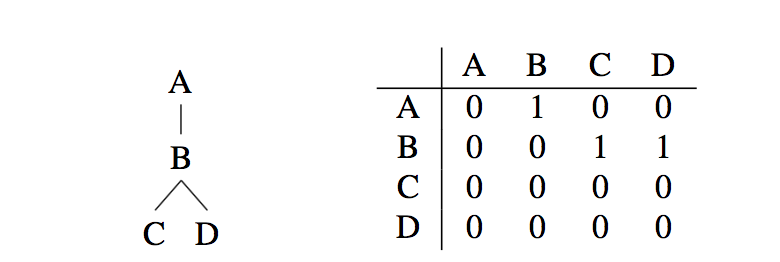
\includegraphics[width=6cm]{./figs/graph-matrix.png}
	\caption{4-graph example: Element of adjacency matrix is a binary string ``0100 0011 0000 0000", for which the decimal number is 17152}
	\label{fig:graph-ex}
	\end{figure}

	\item \textbf{Library Calls} \\
	If call of any contract from any other library occurs in the contract, addresses of all library contracts will be recorded. Similarity among them will be calculated with Jacobian similarity formula.

	\item \textbf{Type Signature} \\
	This feature is composed of input parameter type and return parameter type, and similarity between them can be calculated with Jacobian similarity formula. For example, for the following smart contract code, feature of Type Signature of function ``getBalance" is vector (address, uint256). \\

	\begin{figure}[h]
  	\centering
  	\begin{minipage}{.7\linewidth}
	\begin{lstlisting}[frame=single]
contract addressTest {
  function getBalance(address addr) returns (uint) {
  	return addr.balance;
  }
}
	\end{lstlisting}
  	\end{minipage}
	\end{figure}

	\item \textbf{Local Types:} This feature is the set of all types of local variables of the function body, for which similarity should be calculated with Jacobian similarity formula.

	\item \textbf{Numeric Literals:} The set of all numeric constants serves as the feature of Numeric Literals, for which similarity should be calculated with Jacobian similarity formula.

	\item \textbf{String Literals:} The set of all string constants serves as the feature of String Literals, for which similarity should be calculated with Jacobian similarity formula.
\end{itemize}

Feature family can be expanded, so it is convenient to add new features to it. Based on the circumstance that there is a similarity calculation for each feature, we calculate the weighted sum of all features and thus can acquire the final code similarity:

\begin{equation}
	sim_{combined}(\vec{A}, \vec{B})=\frac{\sum_{c=1}^{n_{cl}}sim_{c}(\vec{A_c},~\vec{B_c})\cdot w_{c}}{\sum_{c=1}^{n_{cl}}w_{c}}
\end{equation}

Therein, $\vec{A}$ and $\vec{B}$ are eigenvectors; $n_{cl}$ is number of features in the feature family; $sim_{c}$ is similarity calculation function specific to feature c; $\vec{A_c}$ and $\vec{B_c}$ are eigenvectors of feature c; $w_{c}$ is weight of c. Weight can be acquired through machine learning algorithm training based on a large number of test sets.